%------------------------------------------%
% Cannabis Data Science
% Saturday Morning Statistics
% Date: 2/26/2022
%------------------------------------------%
\documentclass[xcolor={dvipsnames}]{beamer}
\hypersetup{pdfpagemode = FullScreen}
\mode<presentation>{
  \usetheme{Boadilla}
  \usecolortheme{orchid}
  \usefonttheme{default}
  \setbeamertemplate{navigation symbols}{}
  \setbeamertemplate{caption}[numbered]
}
\setbeamersize{
  text margin left = 0.5in,
  text margin right = 0.5in
}

%------------------------------------------%
% Title
%------------------------------------------%
\author{Cannabis Data Science}
\title[\textbf{Saturday Morning Statistics \#13}]{}
\institute[]{\Large Saturday Morning Statistics \#13}
\date{February \nth{26}, 2022}

%------------------------------------------%
% Packages
%------------------------------------------%
\usepackage[english]{babel}
\usepackage[utf8x]{inputenc}
\usepackage{tikz}
\usepackage{xparse}

%------------------------------------------%
% Colors
%------------------------------------------%
\definecolor{Green}{RGB}{34, 153, 84}
\definecolor{LightGreen}{RGB}{218, 247, 166}
\definecolor{DarkGreen}{RGB}{2, 48, 32}
\definecolor{Orange}{RGB}{255, 87, 51}
\definecolor{DarkOrange}{RGB}{199, 0, 57}
\definecolor{Yellow}{RGB}{255, 195, 0}

%------------------------------------------%
% Theme
%------------------------------------------%
\setbeamercolor*{palette primary}{bg=LightGreen, fg=DarkGreen}
\setbeamercolor*{palette secondary}{bg=LightGreen, fg=DarkGreen}
\setbeamercolor*{palette tertiary}{bg=LightGreen, fg=DarkGreen}

%------------------------------------------%
% Packages
%------------------------------------------%
\usepackage{amsmath}
\renewcommand*\footnoterule{} % No separating line on footnote.
\usepackage{mathtools} % For annotating equations.
\usepackage{hhline} % for double bars.
\usepackage[super]{nth} % For formatting 1st, 2nd, 3rd, etc.
\usepackage{graphicx, caption, subcaption}
\usepackage{setspace}

%------------------------------------------%
% Commands
%------------------------------------------%

% Top space.
\newcommand\T{\rule{0pt}{2.5ex}}

% Bottom space.
\newcommand\B{\rule[-1.25ex]{0pt}{0pt}}

% Blocks.
\newenvironment<>{Block}[2][.9\textwidth]
  {\setlength{\textwidth}{#1}
  \begin{actionenv}#3
    \def\insertblocktitle{#2}\par
    \usebeamertemplate{block begin}}
  {\par\usebeamertemplate{block end}
  \end{actionenv}}

% Balls.
\defbeamertemplate{enumerate item}{largeball}
{\begin{pgfpicture}{-1ex}{-0.65ex}{1.5ex}{1.5ex}
\usebeamercolor[fg]{item projected}
{\pgftransformscale{2.5}\pgftext{\Large\pgfuseshading{bigsphere}}}
{\pgftransformshift{\pgfpoint{0pt}{0.5pt}}
\pgftext{\usebeamerfont*{item projected}\small\insertenumlabel}}
\end{pgfpicture}}

% Fancy arrows.
\NewDocumentCommand\UpArrow{O{2.0ex} O{black}}{%
   \mathrel{\tikz[baseline] \draw [->, line width=0.5pt, #2] (0,0) -- ++(0,#1);}} % Fancy up-arrow.
\NewDocumentCommand\DownArrow{O{2.0ex} O{black}}{%
   \mathrel{\tikz[baseline] \draw [<-, line width=0.5pt, #2] (0,0) -- ++(0,#1);}} % Fancy down-arrow.

% Equations with numbers on the left.
\makeatletter
\newcommand{\LeftEqNo}{\let\veqno\@@leqno}
\makeatother

%------------------------------------------%
% Presentation
%------------------------------------------%
\begin{document}

%------------------------------------------%
% Title Page
%------------------------------------------%
\begin{frame}{}
  
\includegraphics[scale=0.33]{images/logo.pdf}
  \vspace*{-2\baselineskip}
  \titlepage
\end{frame}


% TODO: Introdocue pioneers

% Howard Raiffa
% https://en.wikipedia.org/wiki/Howard_Raiffa

% Robert Schlaifer
% https://en.wikipedia.org/wiki/Robert_Schlaifer

% John P. Craven
% https://en.wikipedia.org/wiki/John_P._Craven

%------------------------------------------%
% Prologue
%------------------------------------------%
\section{Introduction to Distributions}
\begin{frame}{}

{\large \textbf{Pertinent Distributions}}\vspace{\baselineskip}\\

% Normal Distribution
\begin{minipage}{.45\textwidth}
\begin{figure}
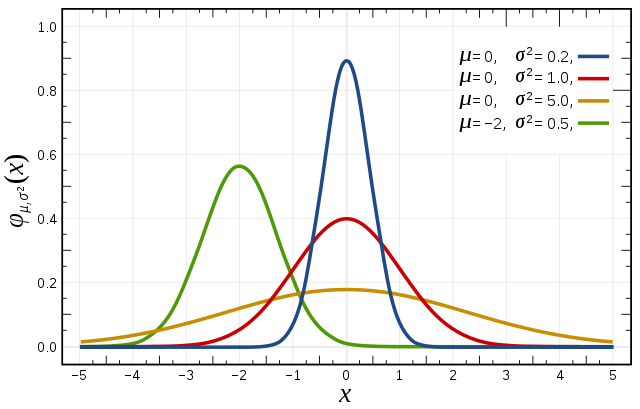
\includegraphics[height=1.1in]{images/normal-distribution.png}
\caption*{%
  \scriptsize
  {\bfseries Normal Distribution}\\[.5\baselineskip]
  Notation: $\mathcal{N}(\mu, \sigma^2)$\\[.5\baselineskip]
  Parameters: mean $\mu \in \mathbb{R}$, \\variance $\sigma^2 \in \mathbb{R}_{>0}$\\[.5\baselineskip]
  PDF:$p(x | \mu, \sigma^2) = \frac{1}{\sigma\sqrt{2\pi}}\text{exp}\left[ -\frac{1}{2}\left( \frac{x - \mu}{\sigma} \right)^2 \right]
$
}
\end{figure}
\end{minipage}\hspace{.05\textwidth}%
% Gamma Distribution
\begin{minipage}{.45\textwidth}
\begin{figure}
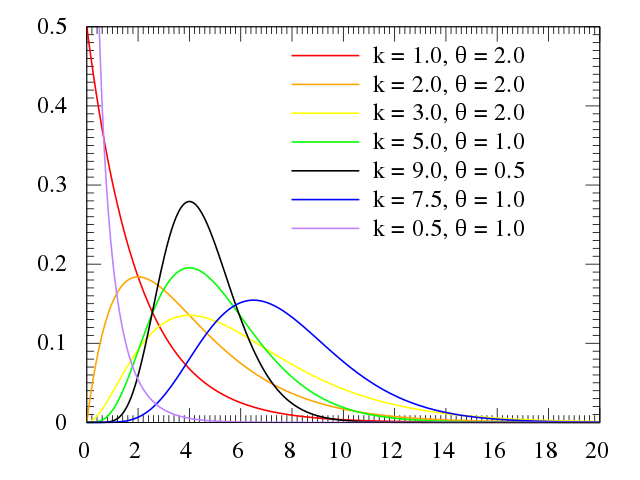
\includegraphics[height=1.1in]{images/gamma-distribution.png}
\caption*{%
  \scriptsize
  {\bfseries Gamma Distribution}\\[.5\baselineskip]
  Notation: $Y \sim G(\alpha, \beta)$\\[.5\baselineskip]
  Parameters: shape $\alpha > 0$, rate $\beta > 0$\\[.5\baselineskip]
  PDF:$
  f_\gamma(y | \alpha, \beta ) \equiv   \begin{cases}
    (\beta^\alpha \Gamma(\alpha))^{-1} y^{\alpha - 1}\text{exp}(-y /\beta)& \text{if } 0 < y < \infty \\
    0 & \text{otherwise.}
\end{cases}$
}
\end{figure}
\end{minipage}

\vfill

{\tiny Gamma Distribution figure credit \\ Authors: MarkSweep and Cburnett \\ License: https://creativecommons.org/licenses/by-sa/3.0/deed.en\\[-1\baselineskip] No changes were made to the figure.}

\end{frame}


\begin{frame}{}

{\large \textbf{Pertinent Distributions - Continued}}\vspace{\baselineskip}\\

% Inverse-gamma Distribution
\begin{minipage}{.3\textwidth}
\begin{figure}
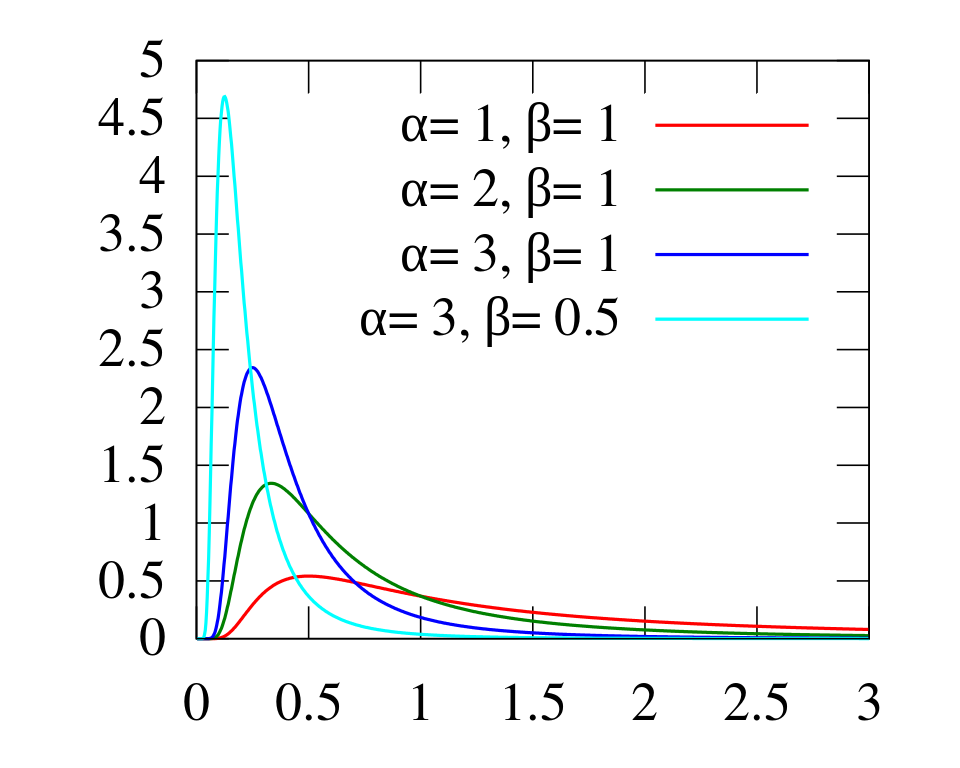
\includegraphics[height=\textwidth]{images/inverse-gamma-distribution.png}
\caption*{%
  \scriptsize
  {\bfseries Inverse-gamma Distribution}\\[.5\baselineskip]
  Notation: $Y \sim \mathcal{IG}(\alpha, \beta)$ \\[.5\baselineskip]
  Parameters: shape $\alpha > 0$, scale $\beta > 0$ \\[.5\baselineskip]
  PDF: $ p(y | \alpha, \beta) = [\Gamma(\alpha)\beta^\alpha]^{-1}y^{-(\alpha + 1)}\text{exp}(-1/[y\beta])$
}
\end{figure}
\end{minipage}\hspace{.15\textwidth}%
% Normal-inverse-gamma Distribution
\begin{minipage}{.55\textwidth}
\begin{figure}
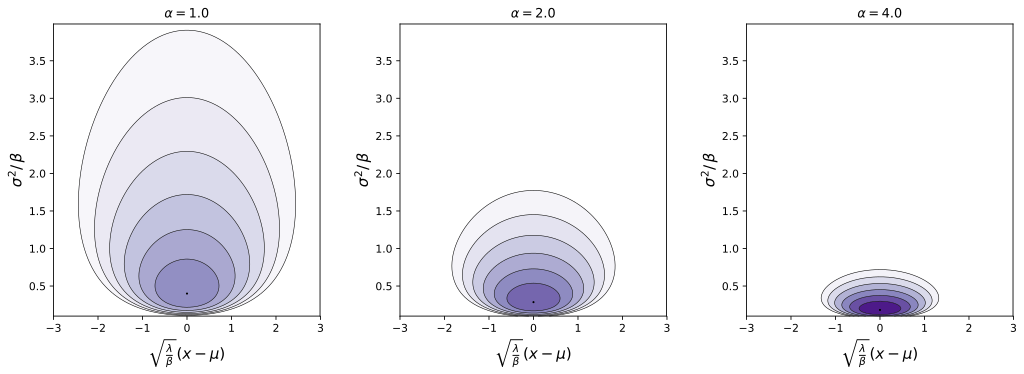
\includegraphics[width=\textwidth]{images/normal-inverse-gamma-distribution.png}
\caption*{%
  \scriptsize
  {\bfseries Normal-inverse-gamma Distribution}\\[.5\baselineskip]
  Notation: $(x, \sigma^2) \sim \mathcal{NIG}(\mu, \lambda, \alpha, \beta)$ \\[.5\baselineskip]
  Parameters: mean $\mu$, variance $\sigma^2/\lambda$, shape $\alpha > 0$, scale $\beta > 0$ \\[.5\baselineskip]
  PDF: $f(x, \sigma^2 | \mu, \lambda, \alpha, \beta) = \frac{\sqrt{\lambda}}{\sqrt{2\pi\sigma^2}}\frac{\beta^\alpha}{\Gamma(\alpha)}\left(\frac{1}{\sigma^2} \right)^{\alpha + 1}\text{exp}\left( -\frac{2\beta + \lambda(x - \mu)^2}{2\sigma^2} \right)$
 }
\end{figure}
\end{minipage}

\vfill
\begin{spacing}{0.5}
  {\tiny Credit: IkamusumeFan (Inverse-gamma distribution figure), Peter.komar.hu (Normal-inverse-gamma distribution figure)\\[.375\baselineskip]
  Licenses: https://creativecommons.org/licenses/by-sa/4.0/deed.en}
\end{spacing}

%{\tiny Gamma Distribution figure credit \\ Authors: MarkSweep and Cburnett \\ License: https://creativecommons.org/licenses/by-sa/3.0/deed.en\\[-1\baselineskip] No changes were made to the figure.}

\end{frame}

%------------------------------------------%
% Multivariate Normal Distribution
%------------------------------------------%
\section{Multivariate Normal Distribution}
\begin{frame}

{\bfseries Multivariate Normal Distribution}\\
\begin{figure}
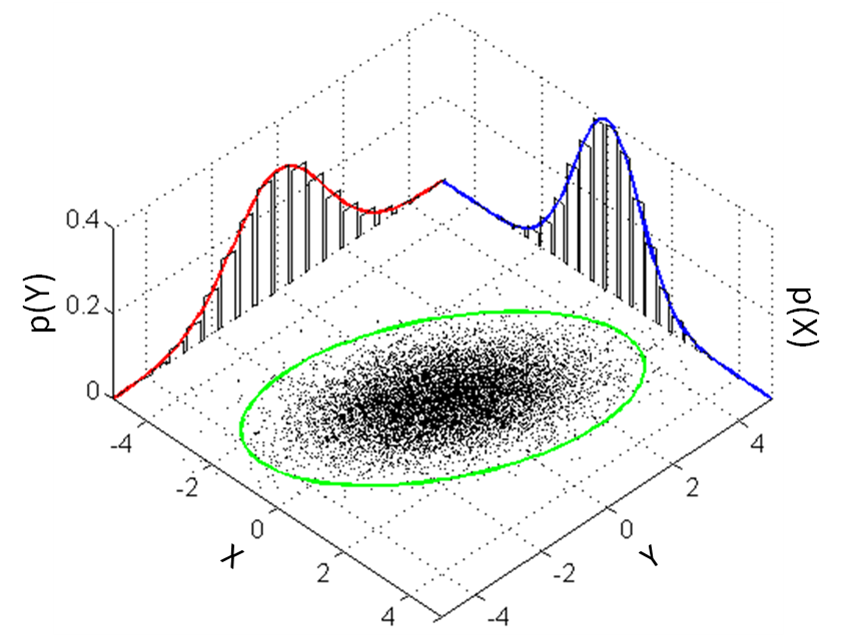
\includegraphics[width=.65\textwidth]{images/multivariate-normal.png}
\caption*{%
  \scriptsize  
  Notation: $Y \sim \mathcal{N}(\mu, \Sigma)$\\[.375\baselineskip]
  Parameters: mean $\mu \in \mathbb{R}^k$, variance $\Sigma \in \mathbb{R}^{k\times k}$\\[.375\baselineskip]
  PDF*: $\phi(y | \mu , \Sigma) = \frac{1}{2\pi^{\frac{k}{2}}}|\Sigma|^{-\frac{1}{2}}\text{exp}\left[-\frac{1}{2}(y - \mu)^\prime\Sigma^{-1}(y-\mu) \right]$
%  $\phi(y | \mu, \sigma) = \text{det}(2\pi\Sigma)^{-\frac{1}{2}}\text{exp}\left[ -\frac{1}{2}  (y - \mu)'\Sigma^{-1}(y - \mu) \right]$
}
\end{figure}

{\scriptsize * The PDF only exists where $\Sigma$ is positive definite.}

\end{frame}

% Optional: Inverse Gamma Distribution

%------------------------------------------%
% Linear Regressions
%------------------------------------------%
\section{Linear Regressions}
\begin{frame}{}

{\large \textbf{Linear Regressions}}\vspace{0.5\baselineskip}\\

Given $i=1,...,N$ observations, the linear regression assumes a linear relationship between the dependent variable, $y_i$, and a vector of $k$ explanatory variables, written as

$$
y = X\beta + \epsilon,
$$

where $y = [y_1 ~ y_2 ~ \cdots ~ y_N]'$ is a $N \times 1$ matrix,

\begin{align*}
X &= \begin{bmatrix}
           x_{1} \\
           x_{2} \\
           \vdots \\
           x_{N}
         \end{bmatrix} \\
\end{align*}


is a $N \times K$ matrix, and $\epsilon = [\epsilon_1 ~ \epsilon_2 ~ \cdots ~ \epsilon_N]'$ is a $N \times 1$ matrix.

\end{frame}

%------------------------------------------%
% Classical Linear Regression
%------------------------------------------%
\section{The Classical Linear Regression}
\begin{frame}{}

{\large \textbf{The Classical Linear Regression}}\vspace{0.5\baselineskip}\\

One of the classical assumption is that errors are {\bfseries normally distributed}

\vspace{-1\baselineskip}
$$
\epsilon \sim \mathcal{N}(0_N, \sigma^2 I_N),
$$

\vspace{0.5\baselineskip}
Assuming a {\bfseries multivariate normal distribution} between $Y$ and $X$, then 

\vspace{-1\baselineskip}
$$
p(y|\beta, h) = \phi (y; X\beta, h^{-1}I_N),
$$

\vspace{0.5\baselineskip}
where $h \equiv \sigma^{-2}$. Assumptions about $\epsilon$ and $X$ define the likelihood function

\vspace{-1\baselineskip}
$$
L(\beta, h) = \frac{h^{\frac{N}{2}}}{(2\pi)^{\frac{N}{2}}}\text{exp}\left[-\frac{h}{2}(y - X\beta)'(y - X\beta)\right].
$$

\vspace{0.5\baselineskip}
The parameters can be estimated by {\bfseries maximum likelihood} or with the {\bfseries ordinary least squares (OLS)} quantities

$$\hat{\beta} = (X^\prime X)^{-1}X^\prime y.$$

\end{frame}

%------------------------------------------%
% The Bayesian Approach to Linear Regressions
%------------------------------------------%
\section{The Bayesian Approach to Linear Regressions}
\begin{frame}{}

{\large \textbf{The Bayesian Approach to Linear Regressions}}\vspace{0.5\baselineskip}\\

The data is assumed to be sampled from a distribution:

$$y \sim \mathcal{N}(\beta^TX, h^{-1} I_N)$$
\vspace{.125\baselineskip}\\

The posterior probability is:

$$P(\beta, h | y, X) = \frac{P(y|\beta, h, X) P(\beta, h | X)}{P(y | X)}$$
\vspace{.125\baselineskip}\\

We can derive the posterior:

$$P(\beta, h | y, X) \propto L(\beta, h)P(\beta, h | X)$$

\end{frame}


\begin{frame}{}

{\large \textbf{Deriving the Bayesian Linear Regression Posterior}}\vspace{0.5\baselineskip}\\

Substituting in the p.d.f.s of the likelihood and our priors allows us to find a closed-form solution

\vspace{-1\baselineskip}
\begin{align*}
P(\beta, h | y) &\propto L(\beta, h)P(\beta, h) \\
P(\beta, h | y) &= \phi(y; X\beta , h^{-1} I_N) \phi(\beta ; \underline{\beta}, h^{-1}\underline{Q})f_\gamma(h | \underline{s}^{-2}, \underline{v})
\end{align*}

where

\vspace{.5\baselineskip}

\begin{itemize}
\item $\underline{\beta}$, $\underline{Q}$, $\underline{s}$, and $\underline{v}$ are hyperparameters of our priors,

\vspace{.5\baselineskip}

\item $\phi()$ is the multivariate normal p.d.f.,

\vspace{.5\baselineskip}

\item $f_\gamma()$ is the gamma density.

\end{itemize}

\vspace{0.5\baselineskip}

The resulting posterior has a {\bfseries normal-gamma} density, we have established {\textit conjugacy}. Our posterior has the same distribution as our prior and our priors are {\bfseries conjugate priors}.

\end{frame}


%------------------------------------------%
% Solving the Bayesian Linear Regression
%------------------------------------------%
\section{Solving the Bayesian Linear Regression}
%\begin{frame}{}
%
%{\large \textbf{Solving the Bayesian Linear Regression}}\vspace{0.5\baselineskip}\\
%
%
%%\begin{align*}
%%
%%\end{align*}
%
%where $\overline{v} = \underline{v} + N$
%
%\end{frame}

\begin{frame}{}

{\large \textbf{Solving the Bayesian Linear Regression}}\vspace{0.5\baselineskip}\\

After substituting the p.d.f.s, our {\bfseries priors} can be found and written in terms of ordinary least squares (OLS) quantities

\vspace*{-0.5\baselineskip}
\begin{align*}
\hat{\beta} &= (X^\prime X)^{-1}X^\prime y\\[0.5\baselineskip]
\overline{Q} &= (\underline{Q}^{-1} + X^\prime X)^{-1}\\[0.5\baselineskip]
\overline{\beta} &= \overline{Q}(\underline{Q}^{-1}\underline{\beta} + X^\prime X \hat{\beta})\\[0.5\baselineskip]
\overline{v}\overline{s}^2 &= \underline{v}\underline{s}^2 + (y - X\hat{\beta})^\prime (y - X\hat{\beta})  + (\hat{\beta} - \underline{\beta})^\prime X^\prime X \overline{Q} \underline{Q}^{-1}(\hat{\beta} - \underline{\beta})
\end{align*}

\vspace*{0.5\baselineskip}
The {\bfseries posterior} distributions are established to be {\bfseries normal-gamma}
\vspace*{-1.0\baselineskip}\\

\begin{align*}
\beta | y, h &\sim \mathcal{N}(\overline{\beta}, h^{-1}\overline{Q}^{-1}) \\[0.5\baselineskip]
h | y &\sim \gamma(\overline{s}^{-2}, \overline{v}).
\end{align*}

\end{frame}

%------------------------------------------%
% The Bayesian Linear Regression Solution
%------------------------------------------%
%\section{The Bayesian Linear Regression Solution}
%\begin{frame}
%
%{\large \textbf{The Bayesian Linear Regression Solution}}\vspace{0.5\baselineskip}\\
%
%The kernel of $\beta | y, h$ is given by
%
%%$$
%%
%%$$
%
%\end{frame}


%------------------------------------------%
% Estimating the Bayesian Linear Regression Solution
%------------------------------------------%
\section{Estimating the Bayesian Linear Regression Solution}
\begin{frame}{}

{\large \textbf{Estimating the Bayesian Linear Regression Solution}}\vspace{0.5\baselineskip}\\

An alternative {\bfseries posterior}  parametrization is with a {\bfseries normal-inverse-gamma} distribution*

\vspace*{-1.0\baselineskip}
\begin{align*}
& \beta | \sigma^2, y \sim \mathcal{N}(\overline{\mu}_\beta, \overline{V}_\beta) \\[0.25\baselineskip]
& \sigma^2 | \beta, y \sim \mathcal{IG}(\overline{a}, \overline{b}).
\end{align*}
\vspace*{-1.25\baselineskip}\\

with hyperparameters $\mu_\beta$, $V_\beta$, $a$,  and $b$ and where

\vspace*{-1.0\baselineskip}
\begin{align*}
\overline{V}_\beta &= \left( \tfrac{X^\prime X}{\sigma^2}+V_\beta^{-1}\right)^{-1} \\[0.25\baselineskip]
\overline{\mu}_\beta &= \overline{V}_\beta \left( \tfrac{X^\prime Y}{\sigma^2} + V_\beta^{-1} \mu_\beta \right) \\[0.25\baselineskip]
\overline{a} &= a + \frac{n}{2} \\[0.25\baselineskip]
\overline{b} &= {\left(\tfrac{1}{b} + \tfrac{1}{2}(Y - X\beta)^\prime (Y - X \beta) \right)}^{-1}.
\end{align*}

\vspace*{-0.25\baselineskip}
\begin{spacing}{0.5}
{\tiny *A theorem states that the inverted gamma distribution has the property that, if $Y$ has an inverted gamma
distribution, then $1/Y$ has a gamma distribution.}
\end{spacing}

\end{frame}

%------------------------------------------%
% Gibbs Sampling
%------------------------------------------%
\section{Gibbs Sampling}
\begin{frame}{}

{\large \textbf{Gibbs Sampling}}\vspace{0.5\baselineskip}\\

Implementing Gibbs sampling to get a random sample from your {\bfseries posterior} entails:

\vspace*{0.5\baselineskip}
\begin{enumerate}

\item Start with an initial value for $\sigma^2$, the desired number of posterior draws, $R$, and the number of burn in draws, $R_0$, sufficient to converge to the posterior distribution.

\vspace*{0.5\baselineskip}

\item Sample $\beta^*$ from the posterior $\beta | \sigma^2, y$.

\vspace*{0.5\baselineskip}

% FIXME: This doesn't make sense.
\item Sample $\sigma^{*2}$ from the posterior $\sigma^2 | \beta = \beta^* y$ given the draw, $\beta^*$.

\vspace*{0.5\baselineskip}

\item Repeat steps (2) and (3) until you have draws for $\beta^*$ and $\sigma^{*2}$ equal to $R + R_0$, the number of desired posterior draws plus the number of burn in draws.

\vspace*{0.5\baselineskip}

\item Drop the first number of burn in draws, $R_0$, for $\beta^*$ and $\sigma^{*2}$.

\end{enumerate}

\end{frame}

%------------------------------------------%
% Takeaway
%------------------------------------------%
\section{Takeaway}
\begin{frame}{}

\begin{center}
\begin{minipage}{3.85in}

% Thank you.
\begin{center}

\includegraphics[width=.25in]{images/prayer.png} {\Large \textbf{Thank you for coming.}}\\
\end{center}
\vspace*{0.5\baselineskip}

% Re-cap the lesson of the week.
\begin{center}
\begin{minipage}{\linewidth}
\begin{Block}{Lesson of the Day}

\vspace{0.5\baselineskip}

\begin{itemize}

\item Bayesian analysis allows us to estimate a distribution for our parameters of interest.

\vspace{0.5\baselineskip}

\end{itemize}

\end{Block}
\end{minipage}
\end{center}

\vspace*{2\baselineskip}

{\bfseries References}\\[-0.75\baselineskip]

Bayesian Econometric Methods,  Koop, Poirier, and Tobias (2007).

\end{minipage}
\end{center}

\end{frame}




%------------------------------------------%
% End
%------------------------------------------%
\end{document}
